%Rapporten har to formål:
%
%
%1.	At give en orientering til DTU-vejlederen om det faglige indhold i praktikken. Dette er gældende også selvom du ikke laver eksamensprojekt i praktikvirksomheden.  Tal med din DTU-vejlederen og lad praktikrapporten være med til at afstemme de fælles forventninger til eksamensprojektet. 
%
%2.	At give en tilbagemelding til praktikkoordinatorerne på den studerendes vurdering af virksomheden som praktikplads. Rapporten læses af praktikkoordinatorerne og arkiveres herefter til senere brug. Tilbagemeldingen anvendes såvel på kort som lang sigt til vurdering af den enkelte virksomheders egnethed som praktikværter.
%Ønsker den studerende at bidrage med mundtlig tilbagemelding, f.eks. om ting som er mere velegnet for en 2 vejs mundtlig kommunikation, skal praktikkoordinatorerne kontaktes. 
%
%Rapporten forventes at have et omfang på mellem 5 og 10 sider.
%
%Du skal være opmærksom på, at arbejde udført i praktikperioden ikke direkte kan indgå som en del af eksamensprojektet. Eksamensprojektet omfatter udelukkende de aktivite-ter der udføres i denne periode.
%Ønsker du at referere til resultater fra praktikperioden, skal det gøres ved at etablere re-sultater fra praktikperioden som rapporter, artikler eller andre former for afsluttede do-kumenter der har dig som forfatter. Disse dokumenter kan du så referere til som bilag til eksamensprojektet.


\documentclass[11pt,a4paper,UKenglish]{article}
% Template by DTU LaTeX support group, v20090423

\usepackage[latin1]{inputenc} % Must correspond to the input encoding used by the editor
\usepackage{babel} % Other languages, in this case UKenglish
\usepackage[T1]{fontenc} % font encoding (output), use T1 for most latin languages
\usepackage{lmodern} % vector based Computer Modern font
\usepackage{graphicx} % for graphics
\graphicspath{{./figures/}} % path to figures and images

\usepackage{mathtools} % mathmatics

\usepackage{xcolor}
\usepackage[plainpages=false,pdfpagelabels,pageanchor=false]{hyperref} % active links
\hypersetup{
  pdfauthor={Kim Rostgaard Christensen},
  pdftitle={Internship report},
  pdfsubject={Internship report},
  citebordercolor={1 1 1}, % The color of the box around citations (change to 1 1 1 to remove)
  linkbordercolor={1 1 1}, % The color of the box around normal links
  pagebordercolor={1 1 1}, % The color of the box around links to pages
  urlbordercolor= {1 1 1}  % The color of the box around links to URLs
}
\usepackage{memhfixc}% fixes for hyperref

% The following can be used if not using custom frontpage
\title{Internship report}
\author{Kim Rostgaard Christensen\\
        \\
        s084283
}
\date{\today}


% \includeonly{preface,assignments,testing} % Only compile those files you are working in (to save compile time, and power)

\begin{document}
%\frontmatter % roman page numbering
\maketitle  % use this if not using custom frontpage
%%%  build with pdflatex
\documentclass[10pt,english]{article}
\renewcommand{\familydefault}{\sfdefault}
\usepackage[T1]{fontenc}
\usepackage[latin9]{inputenc}
\usepackage[letterpaper]{geometry}
\geometry{verbose,tmargin=2.5cm,bmargin=2.5cm,lmargin=2.5cm,rmargin=2.5cm}
\usepackage{array}
\usepackage{amsmath}
\usepackage{graphicx}
\usepackage{amssymb}

\makeatletter

%%%%%%%%%%%%%%%%%%%%%%%%%%%%%% LyX specific LaTeX commands.
%% Because html converters don't know tabularnewline
\providecommand{\tabularnewline}{\\}

%%%%%%%%%%%%%%%%%%%%%%%%%%%%%% User specified LaTeX commands.
\makeatother

\makeatother

\usepackage{babel}

\begin{document}
\begin{flushright}
\textsc{
\includegraphics{fig/dtu_A1_UK}}
\par\end{flushright}

\begin{flushright}
\vspace{1in}

\par\end{flushright}

\begin{center}
{\Huge 02321 Hardware/software programming}
\par\end{center}{\Huge \par}



\begin{center}
{\Large January 20 2011}
\par\end{center}{\Large \par}



\begin{center}
Group 2\\

\par\end{center}

\begin{center}
\begin{tabular}{cr}
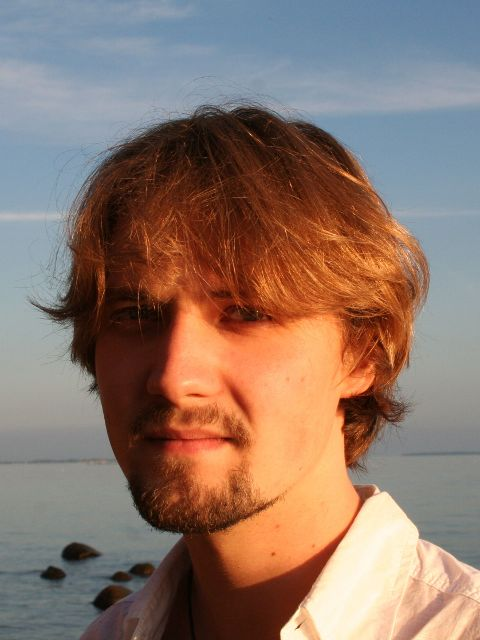
\includegraphics[width=2cm]{img/KRC.jpg} & Kim Rostgaard Christensen (s084283)\tabularnewline
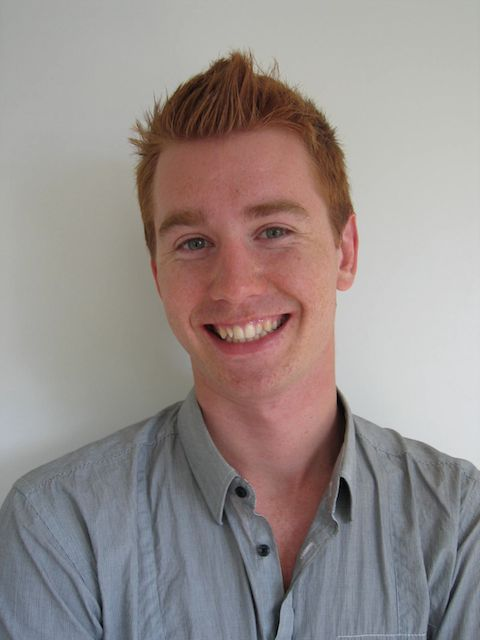
\includegraphics[width=2cm]{img/MHI.jpg} & Morten Hillebo (s072923)\tabularnewline
\end{tabular}
\par\end{center}
\end{document}


\begin{abstract}
This report document my three-months internship with Atkins Denmark. The overall goal of the internship period was to learn about the railway industry with a focus on safety engineering.
\end{abstract}

\tableofcontents
\listoffigures
\listoftables

%\mainmatter % arabic page numbering
\section*{Introduction} 
As part of my engineers degree, it is mandatory for me to have an internship period of 20 weeks.

My internship period is reduced from 20 weeks to 3 (rounded from 10 weeks months due to received merits.\\\\
The defined purpose of the stay was for me to study the theory behind 



\section{Atkins Denmark}
This section contains a brief description of Atkins Denmark, its role in the Atkins Global corporation and the Risk Management department where I was located.


Atkins Denmark is an advisory company that operates within the following areas of expertise:

\begin{itemize}
  \item Transportation - mainly railway
  \item Climate and environment
  \item GIS \& IT
  \item Surveying
  \item Risk Management
  \item Energy
  \item Architecture \& Design
  \item Bridges \& Construction
\end{itemize}
\subsection{Risk Department}
The risk department where I worked is again split into two branches; RAMS and Validation.\\\\
The RAMS department is not surprisingly doing RAMS\footnote{Reliability Availability Maintainability Safety} tasks. Furthermore they do risk assessment, qualitative and quantitative analyses and modelling, including methods design. Last, but not least the also do Human Factors analysis\\\\
The validation department is in charge of validating technical systems, primarily interlocking systems. The department has approved in-house validators.\\\\
Both branches work primarily with railway safety, which is also considered their core competence.

\subsection{Atkins as an internship company}
My impression is that Atkins is very qualified as an internship company. They take very good care of their employees and have a very good working environment.\\\\
For the more hands-on IT interested, they also have the GIS  \& IT department.

\section{Assignments}
Due to the relative short stay at Atkins Risk, I was not able to join an existing project and instead had various tasks outlined in this section.

\subsection{Railway theory and business management}
Although technically not an assignment, I have decided to include this as part of my internship report. This i mainly due to the fact, that I have spent i great deal of time studying the concepts and application of railway technology and application.

I have taken the following two courses during my stay at Atkins.

\begin{itemize}
  \item Introductory railway concepts
  \item Introduction to Business management system
\end{itemize}
The introductory railway course curriculum consisted of topics that covered the different aspects of railway history, planning, construction and maintenance. 

\subsection{Document and technical drawing archiving}
This project was aimed to be a holistic digital archiving solution for paper documents and drawings.\\\\
The concept was to have a three-phase storage process
\begin{itemize}
  \item Scan the document
  \item Archive the document on a net share
  \item Use OCR to auto-tag documents - or provide fulltext search indexes.
\end{itemize}
This project never left the theoretical discussion stage, but was stopped by grounds of questionable usefulness.

\subsection{Defining and documenting a V\&V process}
This project was the main time-consumer of my time. It is a large project, already in progress, which meant that there was a vast quantity of documentation to read through.

This task involved reading though the existing documentation - which was extensive. And Modelling. See section \ref{sec:vandv} for more details


\subsection{Learn concepts and application of FRAM}
The Functional Resonance Analysis Method - or FRAM - is a method developed by Erik Hollnagel. It is a radically different approach to resilience engineering, taking into account human factors as functions in a system.\\\\
FRAM is a method I will be using in my final project.


\section{V\&V application}
This section serves to elaborate on the http based proof of concept constructed.
\subsection{Concept}
The application is meant as a tool for assisting and unifying the process of producing and registering V\&V documentation.\\
\begin{figure}[!tbh]
	\centering
	\includegraphics[width=1.0\textwidth]{img/login.png}
	\caption{Main login screen}
	\label{fig:login}
\end{figure}
The individual stakeholders; in this case typically entrepreneurs, will have to produce documents that proves they have gone though a number of activities outlined for them in a safety plan.\\\\
The system has a classic user-level safety model, each user having a different role in the system. The login screen is depicted in figure \ref{fig:login}.
When the user is logged i, he/she will be presented with a list of pending activities, and some options on what actions to take. This is depicted in figure \ref{fig:main}\\\\
The web-system is a manifestation of a larger data model built during the internship period.
\begin{figure}[!tbh]
	\centering
	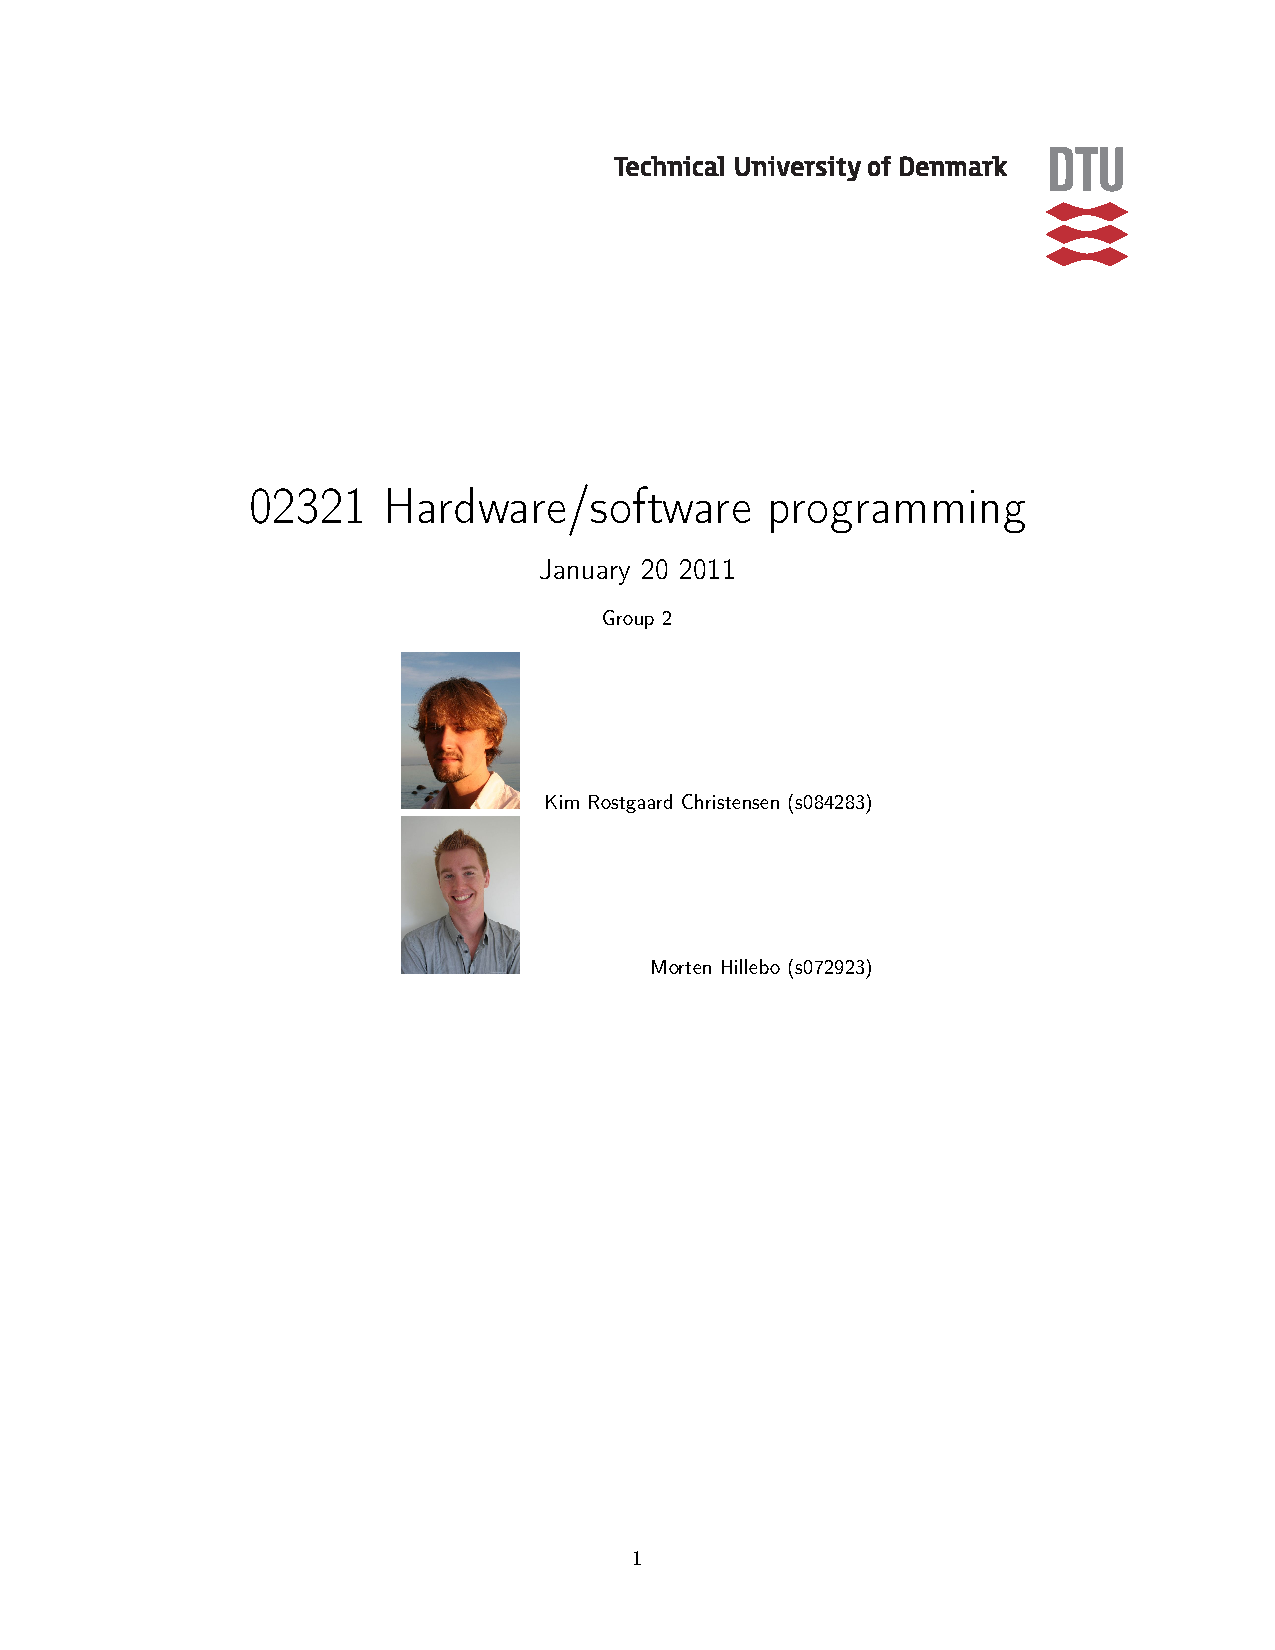
\includegraphics[width=1.0\textwidth]{img/frontpage.png}
	\caption{Home screen}
	\label{fig:main}
\end{figure}

\section{Discussion}
13 weeks has bee too short of a period for an internship. I was explicitly told that I was not able to join any bigger projects on that account - which limited my options, and gains significantly. For the record, my personal opinion is that the internship should either be extended to 20 weeks - or dropped completely for the individuals on a special study plan\\\\
Another impractical issue with 10 weeks, is that is will most likely take 1.5 semester to finish both internship and exam project.

\section{Conclusion}
My stay at Atkins has been a very educational, but also very turbulent experience. I would definitely recommend anyone interested in railways, safety-critical systems, GIS  or anything else within Atkins area of expertise, to  apply for an internship with them.


\bibliographystyle{plain} % pr�v ogs�: is-unsrt, alpha, plain
\bibliography{biblio/template-bib}
%\nocite{*} % \nocite bruges til b�ger som skal med i litteraturlisten
            % men som ikke er refereret til. Alts� baggrundsstof mv.


\appendix % Alphabetic chapter numbering
%\renewcommand{\appendixtocname}{Appendix} % Change appendix name for the table od contents
%\addappheadtotoc % 'Appendix' to the table of contents



%\backmatter % for glossary, index, back page
\end{document}
